\documentclass[a4paper,12pt,reqno]{amsart}
\usepackage{M67tds}

% pour voir les solutions il faut enlever le commentaire de la ligne suivante
% \solutionstrue

\DeclareMathOperator{\aire}{aire}

\begin{document}

% ==================================
\hautdepage{
  \ifsolutions{Solutions du rattrapage}\else{Rattrapage}\fi\par\normalfont\normalsize
  29 juin 2018\\{[ durée: 3 heures ]}\par
}
% ==================================
\ifsolutions\else
  \tikz[baseline=(e.base)]{\NoAutoSpacing\node(e){!};\draw[red,ultra thick,line join=round,yshift=-.15ex](90:1em)--(210:1em)--(330:1em)--cycle;}
  \textbf{Documents autorisés :}\textit{Une feuille A4 recto-verso écrite à la main.}

  \vspace{7mm}
  \tsvp
\fi


%-----------------------------------
\begin{exo}[.7] (Construction à la règle et au compas)

  On se place dans le plan cartésien $\mathbf{R}^2$. Construire à la règle et au compas, à partir des points $O=(0,0)$ et $I=(1,0)$, le point de coordonnées $\displaystyle{(\sqrt{7}, \frac{1}{5})}$. On donnera un programme de construction clair et justifié, accompagné d'un dessin.
\end{exo}

\begin{solution}

  \begin{convention}
    On note $C(X,Y)$ le cercle de centre $X$ passant par $Y$, $C(X,YZ)$ le cercle de centre X et de rayon $YZ$ (qui est constructible si $X$, $Y$ et $Z$ le sont) et $C^{*}(X,Y) = C(X,Y)\setminus\{Y\}$.
  \end{convention}
  \sidebyside{.56}{
    \begin{itemize}
      \item Soit $J(-1,0) = (OI) \cap C^{*}(O,I)$.
      \item Soient $K(0,\sqrt{3})$ et $K'(0,-\sqrt{3})$ les points de $C(I,J) \cap C(J,I)$.
      \item Soit $L(2,0) = (OI) \cap C(I,O)$.
      \item Soit $M(\sqrt{7},0) =  [OI) \cap C(O,KL)$.
      \item Soit $N(4,0) = (OI) \cap C^{*}(L,O)$.
      \item Soit $P(5,0) = (OI) \cap C^{*}(N,OI)$.
      \item Soit $Q(0,1) = (KK') \cap C^{*}(N,OI)$.
    \end{itemize}
  }{
    \raisebox{-49mm}[0pt][0pt]{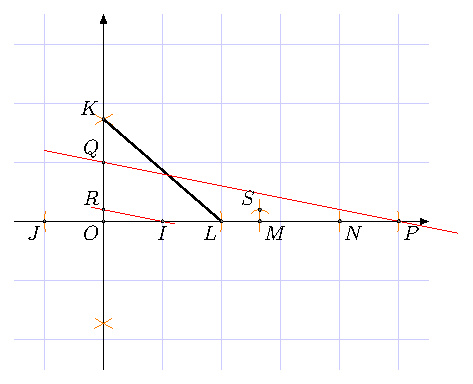
\includegraphics[width=70mm]{M67_2017-18_Rattrapage_img_exo1sol}}
  }
  \begin{itemize}
    \item Soit $\Delta$ la droite qui passe par $I$ et est parallèle à $(PQ)$. Soit $R(0,\frac{1}{5}) = \Delta \cap (KK')$.
    \item Soit $S(\sqrt{7},\frac{1}{5}) = C(M,OR) \cap C(R,OM)$.
  \end{itemize}

\end{solution}


%-----------------------------------
\begin{exo} (Hexagone régulier)

  Soient $\Gamma$ un cercle de centre $O$ et $A_1$ un point de $\Gamma$. Soient $A_2$ et $A_6$ les points d'intersection de $\Gamma$ et du cercle de centre $A_1$ passant par $O$. Le cercle de centre $A_2$ passant par $A_1$ recoupe $\Gamma$ en $A_3$, celui de centre $A_3$ passant par $A_2$ recoupe $\Gamma$ en $A_4$, celui de centre $A_4$ passant par $A_3$ recoupe $\Gamma$ en $A_5$.

  Démontrer que $A_1 A_2 A_3 A_4 A_5 A_6$ est un hexagone régulier, c'est-à-dire un hexagone dont tous les côtés sont de même longueur et dont tous les angles (intérieurs) sont égaux.\\
  \emph{(On ne demande pas de justifier la construction des points $A_1,\ldots,A_6$.)}

\end{exo}

\begin{solution}

  \sidebyside{.7}{
    Par construction, les triangles $A_1OA_2$, $A_6OA_1$, $A_2OA_3$, $A_3OA_4$, $A_4OA_5$ sont équilatéraux. Leurs angles en $O$ sont donc égaux à $\pi/3$. Ainsi, l'angle au sommet du triangle isocèle $A_5OA_6$ vaut $2\pi-5\pi/3=\pi/3$. Le triangle est équilatéral, et les 6 côtés de l'hexagone ont même longueur, égale au rayon du cercle. De plus, les angles $\widehat{A_2A_1A_6}, \widehat{A_3A_2A_1},\ldots,\widehat{A_1A_6A_5}$ sont tous égaux à $2\pi/3$.
  }{
    \raisebox{-42mm}[0pt][0pt]{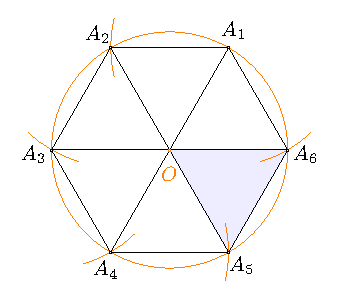
\includegraphics[width=57mm]{M67_2017-18_Rattrapage_img_exo2sol}}
  }

\end{solution}


%-----------------------------------
\begin{exo} (Aire)

  Soient $ABCD$ un rectangle, $I$ le milieu de $[AD]$, $J$ celui de $[CD]$ et $M$ le point d'intersection de $(CI)$ et $(AJ)$.
  \begin{enumerate}
    \item Montrer que $M$ est à l'intérieur du rectangle $ABCD$.\\
    \begin{indication}
      on pourra préciser la nature de $M$ pour le triangle $ACD$.
    \end{indication}
    \item Montrer que $\aire(ABCM)=4\aire(IDJM)$.
  \end{enumerate}

\end{exo}

\begin{solution}

    \begin{enumerate}
      \item Puisque les droites $(IC)$ et $(AJ)$ sont des médianes de $ACD$, $M$ est le centre de gravité de ce triangle. Il est donc à l'intérieur de $ACD$ et a fortiori à l'intérieur du rectangle $ABCD$.
      \item
      \sidebyside{.59}{
        Les triangles $DJM$ et $ABM$ sont homothétiques (image l'un de l'autre par une homothétie de centre $M$; on peut aussi constater que leurs angles sont égaux). Le rapport d'homothétie est égal à $\frac{DM}{BM}$. Or, si $O$ est le milieu de $[AC]$ (qui est celui de $[BD]$, puisque $ABCD$ est un parallélogramme), on a $2 MO= DM=\frac{2}{3}DO$, d'où, puisque $DO=OB$, $\frac{DM}{BM}=\frac{1}{2}$.
      }{
        \raggedleft\raisebox{-42mm}[0pt][0pt]{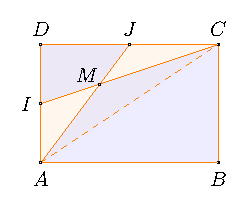
\includegraphics[width=59mm]{M67_2017-18_Rattrapage_img_exo3sol}}
      }\\[3pt]
      Ainsi $\aire{ABM}=2^2\aire{DJM}$. On montre de même que $BCM$ et $DIM$ sont semblables, de rapport $2 \colon 1$, d'où  $\aire{BCM}=2^2\aire{DIM}$. La conclusion en résulte.
    \end{enumerate}
\end{solution}


%-----------------------------------
\begin{exo}\label{heron} (Formule de Héron)

  Soit $ABC$ un triangle. On note $a=BC$, $b=AC$, $c=AB$.
  \begin{enumerate}
    \item\label{loicos} Démontrer que $a^2=b^2+c^2-2bc\cos\widehat{BAC}$.
    \item Exprimer $4b^2c^2\sin^2 \widehat{BAC}$ en fonction de $a$, $b$ et $c$.
    \item En déduire la formule de Héron: l'aire du triangle $ABC$ est égale à $\aire(ABC)=\sqrt{p(p-a)(p-b)(p-c)}$, où $p=\frac{a+b+c}{2}$ est le demi-périmètre du triangle.
    \item Exprimer le rayon du cercle inscrit dans $ABC$ en fonction des longueurs $a$, $b$ et $c$.
  \end{enumerate}
\end{exo}

\begin{solution}

  \begin{enumerate}
    \item Vu en cours.
    \item On a $4b^2c^2\sin^2\widehat A=2bc(1-\cos\widehat{A})\cdot 2bc(1+\cos\widehat{A})=(2bc-b^2-c^2+a^2)(2bc+b^2+c^2-a^2)=(a^2-(b-c)^2)((b+c)^2-a^2)$.
    \item On sait que l'aire est égale à $\frac{1}{2} bc\sin^2\widehat{A}$. Son carré est donc égal à $\frac{1}{16}(a-b+c)(a+b-c)(b+c-a)(b+c+a)=\frac{1}{16}(2p-2b)(2p-2c)(2p-2a)2p=p(p-a)(p-b)(p-c)$.
    \item Soit $I$ le centre du cercle inscrit. Le triangle $ABC$ est réunion presque disjointe des triangles $ABI$, $ACI$ et $BCI$. Les hauteurs de ces triangles issues de $I$ sont des rayons du cercle inscrit. Le rayon $r$ de ce cercle vérifie donc $\aire{ABC}=\frac{1}{2} r\cdot (a+b+c)=rp$. On obtient ainsi $r=\sqrt{\frac{(p-a)(p-b)(p-c)}{p}}$.
  \end{enumerate}
\end{solution}


%------------------------------------
\begin{exo} (Triangle équilatéral)

  Les deux questions sont indépendantes.
  \begin{enumerate}
    \item Soit $ABC$  un triangle équilatéral. Soit $G$ son centre de gravité. Montrer que les cercles circonscrits à $ABC$, $ABG$, $ACG$ et $BCG$ ont le même rayon%
    %\footnote{On peut en fait montrer que dans tout triangle $ABC$ d'orthocentre $H$, les cercles circonscrits aux triangles $ABC$, $ABH$, $ACH$ et $BCH$ sont de même rayon.}
    .
    \item Soit $ABC$ un triangle quelconque.
    \begin{enumerate}
    \item Montrer le \emph{théorème de la médiane}: si $I$ est le milieu de $[BC]$, alors $${AB^2+AC^2=\frac{1}{2}BC^2+2AI^2}.$$ \\
    \begin{indication}
      Vous pouvez introduire le pied $H$ de la hauteur issue de $A$, ou utiliser la question (\ref{loicos}) de l'exercice \ref{heron}.
    \end{indication}
    \item En déduire qu'un triangle est équilatéral si et seulement si son centre de gravité et le centre de son cercle circonscrit coïncident.
  \end{enumerate}
\end{enumerate}
\end{exo}

\begin{solution}

  \begin{enumerate}
  \item Le rayon du cercle circonscrit à $ABC$ est $\frac{AB}{2\sin\widehat{BCA}}$, celui de $ABG$, $\frac{AB}{2\sin\widehat{AGB}}$. Or, $ABC$ étant équilatéral, $\widehat{BCA}=\pi/3$ et $\widehat{BGA}=2\pi/3$. Leurs sinus sont donc égaux, et les cercles circonscrits à $ABC$ et à $ABG$ ont même rayon. Par symétrie, c'est aussi le rayon des cercles circonscrits à $ACG$ et $BCG$ (et ce rayon est égal à $\frac{AB}{2\sin(\pi/3)}=\frac{AB}{\sqrt{3}}$.
  \item
  \begin{enumerate}
    \item La loi des cosinus (exercice \ref{heron} (\ref{loicos})) dans $ABI$ s'écrit $AB^2=BI^2+AI^2-2 AI \cdot BI \cos\widehat{AIB}$. Dans $ACI$, on  a de même $AC^2=CI^2+AI^2 - 2 AI \cdot CI \cos \widehat{ACI}$. Les angles $\widehat{AIB}$ et $\widehat{AIC}$ sont supplémentaires, donc leur cosinus sont opposés. En sommant les deux égalités précédentes et en utilisant $BC=2IC=2IB$, on obtient ainsi $AB^2+AC^2=\frac{1}{2}BC^2+2AI^2$.
    \item Dans un triangle équilatéral, les médianes et les médiatrices sont confondues, donc leurs points d'intersection sont les mêmes. Réciproquement, soit $ABC$ un triangle dont le centre de gravité $G$ est le centre du cercle circonscrit. On a alors $AG=BG=CG$. Soient $I,J,K$ les milieux de $[BC]$, $[AC]$ et $[AB]$. Les médianes ont pour longueurs $AI=\frac{3}{2}AG$, $BJ=\frac{3}{2}BG$ et $CK=\frac{3}{2}CG$. Elles sont donc égales. Le théorème de la médiane assure
    \begin{equation*}
      \left\lbrace \begin{array}{rcl} AB^2+AC^2&=&\frac{1}{2}BC^2+2AI^2 \\ AB^2+BC^2&=&\frac{1}{2}AC^2+2BJ^2 \\ AC^2+BC^2&=&\frac{1}{2}AB^2+2CK^2\end{array} \right.
    \end{equation*}
    d'où on déduit $AB^2=\frac{4}{3}AI^2=AC^2=BC^2$. Le triangle $ABC$ est donc équilatéral.
   \end{enumerate}
 \end{enumerate}
\end{solution}


%-----------------------------------
\begin{exo}[.7] (Kangourou 2012)

  \sidebyside{.7}{
    Soient un triangle rectangle de côtés $5$, $12$ et $13$ et le cercle centré sur le côté de longueur $12$ et tangent aux deux autres côtés.\\
    Déterminer le rayon du cercle.
  }{
    \raisebox{-17mm}[0pt][0pt]{\includegraphics[width=5cm]{img_kangourou2012}}
  }
\end{exo}

\begin{solution}

  \sidebyside{.7}{
    On note $O$ le centre du cercle sur le côté $AB$ du triangle $\tri ABC$ et $P$ son point de tangence avec $AC$. Soit le rayon $r=OP=OB$. Nous avons les triangles rectangles semblables $\tri APO$ et $\tri ABC$, et donc $OP:AO=CB:AC$. Ainsi $\frac{r}{12-r}=\frac{5}{13} \iff r=\frac{10}{3}$.
  }{
    \raisebox{-21mm}[0pt][0pt]{\includegraphics[width=5cm]{img_kangourou2012a}}
  }
\end{solution}


\end{document}
